% Provenance (never printed): see sources/outline_sources.md (Year 1:
% astronomy of position, spherical trigonometry, time scales, insolation).
% Spherical trigonometry is absent from the mathematics series: this chapter
% owns it. Curves computed in figdata/bachelor-1/{sun_paths, day_length,
% celestial_sphere, spherical_triangle}.py (shared model _solar.py); numbers
% of the exercises and problem in the Book 3 scratch calculator ch01.py.
\chapter{Astronomie sphérique}\label{ch:b1:spherical-astronomy}

Par une nuit claire, loin de toute ville, un appareil photographique en pose
longue pointé vers le ciel enregistre les étoiles sous la forme d'arcs de
cercle, tous centrés sur un même point qui ne bouge pas. Une étoile qui s'est
levée à l'est à neuf heures ce soir se lèvera demain vers neuf heures moins
cinq, et un peu plus tôt chaque nuit suivante. À midi, le Soleil est plus haut
en juin qu'en décembre, et, à l'extrême nord, il ne se couche pas du tout au
milieu de l'été. Tout cela est la rotation de la Terre et sa révolution
autour du Soleil, vues du sol. Pour le décrire, l'astronome et le
géoscientifique ont besoin de coordonnées sur une sphère, de la
trigonométrie des triangles tracés sur une sphère et d'horloges qui suivent
le rythme des étoiles ou celui du Soleil. Ce chapitre construit ces outils.
Ils reviendront dans la cinématique des plaques
(\cref{ch:b1:plate-kinematics}), où les plaques tournent sur la sphère, et
dans les chapitres sur le climat (\cref{ch:b1:radiation-heat-transport}), où
la lumière que reçoit une \omterm{def:b1:spherical-astronomy:geographic}{latitude} entraîne les vents et les courants.

\begin{recall}
La Terre tourne sur elle-même en un jour et fait le tour du Soleil en un an
sur une orbite presque circulaire~; son axe est incliné par rapport à
l'orbite, ce qui produit les saisons (les livres de physique, années~6 et 12~;
les lois de Kepler sont rappelées du volume de physique de première année).
Un point de la Terre est repéré par sa \omterm{def:b1:spherical-astronomy:geographic}{latitude} et sa \omterm{def:b1:spherical-astronomy:geographic}{longitude} (livre~1,
année~6). Un vecteur de longueur un est fixé par deux angles, comme en
coordonnées sphériques~; le produit scalaire de deux vecteurs unitaires est le
cosinus de l'angle qu'ils forment, et le produit mixte
$\vec u\cdot(\vec v\times\vec w)$ est inchangé par une permutation
circulaire des trois vecteurs.
\end{recall}

\section{Triangles sur la sphère}

\begin{definition}[Grand cercle, triangle sphérique]\label{def:b1:spherical-astronomy:spherical-triangle}
Un \emph{grand cercle}\index{grand cercle} d'une sphère est son intersection
avec un plan passant par son centre~; toute autre section plane est un
\emph{petit cercle}\index{petit cercle}. Par deux points qui ne sont pas
diamétralement opposés passe un seul grand cercle, et le plus court de ses
deux arcs est le plus court chemin sur la sphère entre ces points. Un
\emph{triangle sphérique}\index{triangle sphérique} est la figure formée par
trois points de la sphère, ses sommets $A$, $B$, $C$, joints par des arcs de
grand cercle de longueur angulaire inférieure à \ang{180}. Ses côtés $a$, $b$,
$c$ (opposés à $A$, $B$, $C$) se mesurent par les angles qu'ils sous-tendent au
centre~; ses angles $A$, $B$, $C$ sont les angles entre les plans des côtés
qui se rencontrent à chaque sommet.
\end{definition}

Sur la sphère de rayon $R$, un côté de $a$ radians a pour longueur $Ra$. Tout
côté et tout angle est compris entre $0$ et $\pi$.

\begin{omfigure}
\begin{tikzpicture}
\begin{axis}[x=1cm, y=1cm, hide axis, xmin=-2.7, xmax=2.7, ymin=-2.6, ymax=2.6, clip=false]
\draw[black, line width=0.6pt] (axis cs:0,0) circle (2.4cm);
\addplot[black!45, densely dashed, line width=0.4pt] coordinates {(0,0) (-0.078358,1.7847)};
\addplot[black!45, densely dashed, line width=0.4pt] coordinates {(0,0) (-1.5903,-0.2902)};
\addplot[black!45, densely dashed, line width=0.4pt] coordinates {(0,0) (1.4453,-0.16381)};
\addplot[omDef, line width=1.1pt] table {figdata/out/bachelor-1-spherical_triangle-ab.dat};
\addplot[omDef, line width=1.1pt] table {figdata/out/bachelor-1-spherical_triangle-bc.dat};
\addplot[omDef, line width=1.1pt] table {figdata/out/bachelor-1-spherical_triangle-ca.dat};
\addplot[omThm, line width=0.8pt] table {figdata/out/bachelor-1-spherical_triangle-angA.dat};
\addplot[only marks, mark=*, mark size=1.4pt] table[x=x, y=y] {figdata/out/bachelor-1-spherical_triangle-verts.dat};
\fill (axis cs:0,0) circle (1.2pt);
\begin{scope}[font=\small]
  \node[above] at (axis cs:-0.078358,1.7847) {$A$};
  \node[left] at (axis cs:-1.5903,-0.2902) {$B$};
  \node[right] at (axis cs:1.4453,-0.16381) {$C$};
  \node[above left] at (axis cs:0,0) {$O$};
  \node[omThm] at (axis cs:0.24,1.36) {$A$};
  \node[omDef] at (axis cs:0.0,-0.52) {$a$};
  \node[omDef] at (axis cs:0.95,0.95) {$b$};
  \node[omDef] at (axis cs:-1.05,0.95) {$c$};
\end{scope}
\end{axis}
\end{tikzpicture}

{\small Un \omterm{def:b1:spherical-astronomy:spherical-triangle}{triangle sphérique} $ABC$ sur une sphère de centre $O$. Les côtés
$a$, $b$, $c$ sont des arcs de \omterm{def:b1:spherical-astronomy:spherical-triangle}{grand cercle}, mesurés par les angles $BOC$,
$COA$, $AOB$~; l'angle $A$ (en rouge) est l'angle entre les deux côtés qui se
rencontrent en $A$. Le triangle dessiné a $a = \ang{78.6}$, $b = \ang{62.6}$,
$c = \ang{64.8}$ et des angles de \ang{89.9}, \ang{64.9} et \ang{67.4}, dont
la somme dépasse \ang{180}.}
\end{omfigure}

\begin{theorem}[Formule des cosinus]\label{thm:b1:spherical-astronomy:cosine-rule}
Dans un \omterm{def:b1:spherical-astronomy:spherical-triangle}{triangle sphérique},
\[
  \cos a = \cos b\cos c + \sin b\sin c\cos A .
\]
\end{theorem}

\begin{proof}
On travaille sur la sphère unité et l'on choisit des axes avec $A$ au pôle~:
$\vec A = (0, 0, 1)$, et le plan $xz$ contenant $B$~:
$\vec B = (\sin c, 0, \cos c)$, puisque $B$ est à la distance angulaire $c$ de
$A$. Le point $C$ est à la distance angulaire $b$ de $A$, sur un \omterm{def:b1:spherical-astronomy:spherical-triangle}{grand cercle}
passant par $A$ et faisant l'angle $A$ avec le plan $xz$~:
$\vec C = (\sin b\cos A, \sin b\sin A, \cos b)$. Le côté $a$ est l'angle
entre $\vec B$ et $\vec C$, donc
\[
  \cos a = \vec B\cdot\vec C = \sin c\sin b\cos A + \cos c\cos b. \qedhere
\]
\end{proof}

\begin{theorem}[Formule des sinus]\label{thm:b1:spherical-astronomy:sine-rule}
Dans un \omterm{def:b1:spherical-astronomy:spherical-triangle}{triangle sphérique},
\[
  \frac{\sin A}{\sin a} = \frac{\sin B}{\sin b} = \frac{\sin C}{\sin c}.
\]
\end{theorem}

\begin{proof}
Avec les vecteurs de la démonstration précédente, un calcul direct donne
$\vec B \times \vec C = (-\cos c\sin b\sin A,\ \cos c\sin b\cos A - \sin c\cos b,\
\sin c\sin b\sin A)$, donc le produit mixte vaut
$\vec A\cdot(\vec B\times\vec C) = \sin b\sin c\sin A$. Le produit mixte est
inchangé par une permutation circulaire de $A$, $B$, $C$~; en plaçant $B$, puis
$C$, au pôle, on obtient de la même façon $\sin c\sin a\sin B$ et $\sin a\sin b\sin
C$. Les trois expressions sont égales~; la division par $\sin a\sin b\sin c$
donne la formule.
\end{proof}

Lorsque les côtés sont petits devant le rayon, $\cos a \approx 1 -
a^2/2$ et $\sin a \approx a$, et les deux formules deviennent les formules des
cosinus et des sinus des triangles plans~: sur une portion assez petite, la
sphère est plate. Sur un grand triangle il n'en est rien~: la somme des angles
d'un \omterm{def:b1:spherical-astronomy:spherical-triangle}{triangle sphérique} dépasse \ang{180} (\cref{exo:b1:spherical-astronomy:12}).

\begin{method}[Distance et cap sur la sphère]\label{met:b1:spherical-astronomy:great-circle}
Pour trouver la plus courte distance entre deux lieux de \omterm{def:b1:spherical-astronomy:geographic}{latitudes} $\varphi_1$,
$\varphi_2$ et de \omterm{def:b1:spherical-astronomy:geographic}{longitudes} $\lambda_1$, $\lambda_2$, et la direction dans
laquelle partir~:
\begin{enumerate}
  \item former le triangle dont les sommets sont le pôle Nord $P$ et les deux
        lieux~; ses côtés issus du pôle sont les colatitudes $\ang{90} -
        \varphi_1$ et $\ang{90} - \varphi_2$, et son angle au pôle est
        la différence de \omterm{def:b1:spherical-astronomy:geographic}{longitude} $\Delta\lambda$~;
  \item la formule des cosinus donne la distance angulaire $\Delta$~:
        $\cos\Delta = \sin\varphi_1\sin\varphi_2 +
        \cos\varphi_1\cos\varphi_2\cos\Delta\lambda$~; la distance est
        $R\Delta$ ($\Delta$ en radians)~;
  \item le cap initial est l'angle du triangle au premier lieu, tiré de la
        formule des cosinus appliquée au côté qui lui est opposé,
        $\sin\varphi_2 = \sin\varphi_1\cos\Delta + \cos\varphi_1\sin\Delta\cos
        \mathrm{Az}$, et se mesure depuis le nord vers le second lieu.
\end{enumerate}
Le cap change le long du \omterm{def:b1:spherical-astronomy:spherical-triangle}{grand cercle} (sauf le long d'un méridien ou de
l'équateur)~: un navire ou un avion qui garde le même cap au compas suit une
autre courbe, plus longue.
\end{method}

\section{Coordonnées sur la sphère}

\begin{definition}[Latitude et longitude]\label{def:b1:spherical-astronomy:geographic}
Considérons la Terre comme une sphère tournant autour de son axe polaire. La
\emph{latitude}\index{latitude} $\varphi$ d'un point est l'angle entre
le plan équatorial et le rayon passant par ce point, de \ang{-90}
(pôle Sud) à \ang{+90} (pôle Nord)~; sa \emph{longitude}\index{longitude}
$\lambda$ est l'angle, mesuré dans le plan équatorial, entre le demi-plan
méridien du point et celui d'un méridien de référence, celui de Greenwich,
compté positivement vers l'est, de \ang{-180} à
\ang{180}.
\end{definition}

En réalité, la Terre est légèrement aplatie~; la \omterm{def:b1:spherical-astronomy:geographic}{latitude} employée pour les
cartes et pour le ciel est l'angle entre la verticale du lieu et le plan
équatorial, qui diffère de l'angle géocentrique d'au plus \ang{0.2}
(\cref{ch:b1:isostasy-gravity}). Les lignes d'égale \omterm{def:b1:spherical-astronomy:geographic}{latitude}, les parallèles,
sont des \omterm{def:b1:spherical-astronomy:spherical-triangle}{petits cercles}~; les méridiens sont des moitiés de \omterm{def:b1:spherical-astronomy:spherical-triangle}{grands cercles}.

\begin{definition}[La sphère céleste]\label{def:b1:spherical-astronomy:celestial-sphere}
La \emph{sphère céleste}\index{sphere celeste@sphère céleste} est une sphère
imaginaire centrée sur l'observateur, sur laquelle chaque étoile est placée
dans sa direction~; seules comptent les directions, non les distances. Les
prolongements de l'axe de la Terre la rencontrent aux \emph{pôles
célestes}\index{pole celeste@pôle céleste} nord et sud~; le plan de
l'équateur terrestre la coupe selon l'\emph{équateur
céleste}\index{equateur celeste@équateur céleste}. Le \emph{zénith}\index{zenith@zénith}
est le point situé à la verticale du lieu~; l'horizon est le \omterm{def:b1:spherical-astronomy:spherical-triangle}{grand
cercle} situé à $\ang{90}$ de ce point. Le \emph{méridien du
lieu}\index{meridien du lieu@méridien du lieu} est le \omterm{def:b1:spherical-astronomy:spherical-triangle}{grand cercle} passant par le zénith et les pôles
célestes~; il rencontre l'horizon aux points nord et sud.
\end{definition}

Comme la Terre tourne d'ouest en est, la \omterm{def:b1:spherical-astronomy:celestial-sphere}{sphère céleste} semble tourner dans
l'autre sens, d'est en ouest, autour de l'axe des \omterm{def:b1:spherical-astronomy:celestial-sphere}{pôles célestes}, en un peu
moins d'un jour. Les étoiles gardent leurs positions relatives~: elles sont si
lointaines qu'un voyage d'un an autour du Soleil modifie leurs directions de
moins d'une seconde d'arc (\cref{ch:b1:observing-the-sky}).

\begin{definition}[Coordonnées horizontales]\label{def:b1:spherical-astronomy:horizontal}
La \emph{hauteur}\index{hauteur (d'un astre)} $h$ d'une étoile est son angle
au-dessus de l'horizon, de \ang{-90} à \ang{90}~; sa distance zénithale est
$z = \ang{90} - h$. Son \emph{azimut}\index{azimut} $\mathrm{A}$ est
l'angle, le long de l'horizon, entre le point nord et le pied du cercle
vertical de l'étoile, compté de \ang{0} à \ang{360} en passant par l'est.
\end{definition}

Les coordonnées horizontales sont celles de l'observateur~: elles changent
avec le lieu et l'heure. Les coordonnées du ciel lui-même sont entraînées par
sa rotation.

\begin{definition}[Coordonnées équatoriales]\label{def:b1:spherical-astronomy:equatorial}
La \emph{déclinaison}\index{declinaison (celeste)@déclinaison (céleste)}
$\delta$ d'une étoile est son angle à l'\omterm{def:b1:spherical-astronomy:celestial-sphere}{équateur céleste}, positif vers le
nord, de \ang{-90} à \ang{90}. Le \omterm{def:b1:spherical-astronomy:spherical-triangle}{grand cercle} passant par l'étoile et les
\omterm{def:b1:spherical-astronomy:celestial-sphere}{pôles célestes} est son cercle horaire. L'\emph{angle horaire}\index{angle horaire} $H$ de
l'étoile est l'angle au \omterm{def:b1:spherical-astronomy:celestial-sphere}{pôle céleste} entre le \omterm{def:b1:spherical-astronomy:celestial-sphere}{méridien du lieu} et le cercle
horaire de l'étoile, compté vers l'ouest, en heures de \ang{15}.
L'\emph{ascension droite}\index{ascension droite} $\alpha$ est l'angle le long de l'\omterm{def:b1:spherical-astronomy:celestial-sphere}{équateur céleste},
depuis un point fixe du ciel, le \omterm{def:b1:spherical-astronomy:ecliptic}{point vernal}
(\cref{def:b1:spherical-astronomy:ecliptic}), jusqu'au cercle horaire de
l'étoile, compté vers l'est, également en heures.
\end{definition}

La \omterm{def:b1:spherical-astronomy:equatorial}{déclinaison} et l'\omterm{def:b1:spherical-astronomy:equatorial}{ascension droite} sont fixes sur le ciel, comme la \omterm{def:b1:spherical-astronomy:geographic}{latitude}
et la \omterm{def:b1:spherical-astronomy:geographic}{longitude} sur la Terre~: les catalogues les donnent. Le mot \omterm{def:b1:spherical-astronomy:equatorial}{déclinaison}
n'est employé ici que dans ce sens astronomique~; l'angle entre le nord
géographique et le nord d'une boussole s'appelle toujours la déclinaison
magnétique (\cref{ch:b1:field-lab-methods-1}).

\begin{proposition}[Des coordonnées équatoriales aux coordonnées horizontales]\label{prop:b1:spherical-astronomy:transform}
À la \omterm{def:b1:spherical-astronomy:geographic}{latitude} $\varphi$, une étoile de \omterm{def:b1:spherical-astronomy:equatorial}{déclinaison} $\delta$ et d'\omterm{def:b1:spherical-astronomy:equatorial}{angle horaire}
$H$ a la \omterm{def:b1:spherical-astronomy:horizontal}{hauteur} et l'\omterm{def:b1:spherical-astronomy:horizontal}{azimut} donnés par
\[
  \sin h = \sin\varphi\sin\delta + \cos\varphi\cos\delta\cos H,
  \qquad
  \cos\mathrm{A} = \frac{\sin\delta - \sin\varphi\sin h}{\cos\varphi\cos h},
\]
avec $\mathrm{A}$ compris entre \ang{0} et \ang{180} quand l'étoile est à l'est
du méridien ($\sin H < 0$) et $\mathrm{A} = \ang{360} - \arccos(\dots)$ quand
elle est à l'ouest. En particulier, la \omterm{def:b1:spherical-astronomy:horizontal}{hauteur} du \omterm{def:b1:spherical-astronomy:celestial-sphere}{pôle céleste} nord est égale à
la \omterm{def:b1:spherical-astronomy:geographic}{latitude}.
\end{proposition}

\begin{proof}
Considérons le triangle formé par le \omterm{def:b1:spherical-astronomy:celestial-sphere}{pôle céleste} nord $P$, le \omterm{def:b1:spherical-astronomy:celestial-sphere}{zénith} $Z$
et l'étoile $X$ (le triangle astronomique, ou triangle de position). La
verticale du lieu fait l'angle $\varphi$ avec le plan équatorial, donc $PZ =
\ang{90} - \varphi$~; $PX = \ang{90} - \delta$~; $ZX = \ang{90} - h$. L'angle
en $P$ est l'\omterm{def:b1:spherical-astronomy:equatorial}{angle horaire} $H$~; l'angle en $Z$ est l'\omterm{def:b1:spherical-astronomy:horizontal}{azimut} de l'étoile
mesuré depuis le nord (à l'est ou à l'ouest du méridien). La formule des
cosinus pour le côté $ZX$, opposé à $P$, donne
$\cos(\ang{90} - h) = \cos(\ang{90} - \varphi)\cos(\ang{90} - \delta) +
\sin(\ang{90} - \varphi)\sin(\ang{90} - \delta)\cos H$, c'est-à-dire la première
formule. La formule des cosinus pour le côté $PX$, opposé à $Z$, donne
$\sin\delta = \sin\varphi\sin h + \cos\varphi\cos h\cos\mathrm{A}$, c'est-à-dire
la seconde. Pour le pôle, $\delta = \ang{90}$ et la première formule s'écrit
$\sin h = \sin\varphi$.
\end{proof}

\begin{omfigure}
\begin{tikzpicture}
\pic (cs) at (0,0) {celestialsphere=45};
\begin{axis}[x=1cm, y=1cm, hide axis, anchor=origin, at={(0,0)}, xmin=-2.6, xmax=2.6, ymin=-2.4, ymax=2.5, clip=false]
\addplot[omField, line width=1.1pt] table[x=x, y=y] {figdata/out/bachelor-1-celestial_sphere-vertical.dat};
\addplot[black!80, line width=0.9pt, densely dash dot] table[x=x, y=y] {figdata/out/bachelor-1-celestial_sphere-hourcircle.dat};
\addplot[only marks, mark=star, mark size=3pt, mark options={line width=0.8pt}] table[x=x, y=y] {figdata/out/bachelor-1-celestial_sphere-star.dat};
\end{axis}
\begin{scope}[font=\footnotesize]
  \node[above] at (cs-Z) {$Z$};
  \node[above left] at (cs-NCP) {$P$};
  \node[left] at (cs-N) {N};
  \node[right] at (cs-S) {S};
  \node[below] at (cs-W) {O};
  \node[below, fill=white, fill opacity=0.8, text opacity=1, inner sep=1pt] at (cs-E) {E};
  \node[above right] at (0.2262,0.94) {$X$};
  \node[omField] at (0.55,0.2) {$h$};
  \node[omDef, right] at (2.0,-1.25) {équateur};
  \node[left] at (-2.0,-0.3) {horizon};
  \node at (-1.35,0.62) {$\varphi$};
\end{scope}
\draw[black!60, line width=0.4pt] (-1.05,0) arc[start angle=180, end angle=137, radius=1.05cm];
\end{tikzpicture}

{\small Le ciel à la \omterm{def:b1:spherical-astronomy:geographic}{latitude} \ang{45}~N, vu de l'ouest, le nord à gauche.
Le \omterm{def:b1:spherical-astronomy:celestial-sphere}{pôle céleste} nord $P$ se trouve à une \omterm{def:b1:spherical-astronomy:horizontal}{hauteur} égale à la \omterm{def:b1:spherical-astronomy:geographic}{latitude} au-dessus
du point nord (en rouge~: l'axe des \omterm{def:b1:spherical-astronomy:celestial-sphere}{pôles célestes})~; l'\omterm{def:b1:spherical-astronomy:celestial-sphere}{équateur céleste} (en
bleu) coupe l'horizon aux points est et ouest. Une étoile $X$ de \omterm{def:b1:spherical-astronomy:equatorial}{déclinaison}
\ang{25}, trois heures vingt minutes après son passage au méridien (\omterm{def:b1:spherical-astronomy:equatorial}{angle
horaire} \ang{50}), est à la \omterm{def:b1:spherical-astronomy:horizontal}{hauteur} $h = \ang{45.3}$ (en vert~: son cercle
vertical, du \omterm{def:b1:spherical-astronomy:celestial-sphere}{zénith} $Z$ à l'horizon) et à l'\omterm{def:b1:spherical-astronomy:horizontal}{azimut} \ang{261}~; son cercle
horaire (en tirets et points) va du pôle à l'étoile, puis à l'équateur.
Calculé avec la \cref{prop:b1:spherical-astronomy:transform}.}
\end{omfigure}

\begin{proposition}[Culmination et étoiles circumpolaires]\label{prop:b1:spherical-astronomy:culmination}
À la \omterm{def:b1:spherical-astronomy:geographic}{latitude} $\varphi$, une étoile de \omterm{def:b1:spherical-astronomy:equatorial}{déclinaison} $\delta$ traverse le
méridien ($H = 0$) à la \omterm{def:b1:spherical-astronomy:horizontal}{hauteur} $\ang{90} - |\varphi - \delta|$, au sud du
\omterm{def:b1:spherical-astronomy:celestial-sphere}{zénith} si $\delta < \varphi$, au nord si $\delta > \varphi$. Dans
l'hémisphère nord ($\varphi > 0$), elle ne se couche jamais si
$\delta > \ang{90} - \varphi$ et ne se lève jamais si
$\delta < -(\ang{90} - \varphi)$.
\end{proposition}

\begin{proof}
Pour $H = 0$, $\sin h = \sin\varphi\sin\delta + \cos\varphi\cos\delta =
\cos(\varphi - \delta)$, donc $h = \ang{90} - |\varphi - \delta|$. La \omterm{def:b1:spherical-astronomy:horizontal}{hauteur}
la plus basse, pour $H = \ang{180}$, vérifie $\sin h = -\cos(\varphi + \delta)$~;
elle est positive lorsque $\varphi + \delta > \ang{90}$. L'étoile reste sous
l'horizon lorsque même sa \omterm{def:b1:spherical-astronomy:horizontal}{hauteur} maximale est négative,
$|\varphi - \delta| > \ang{90}$.
\end{proof}

\begin{definition}[Étoile circumpolaire]\label{def:b1:spherical-astronomy:circumpolar}
Une \emph{étoile circumpolaire}\index{etoile circumpolaire@étoile circumpolaire} est une étoile qui ne se couche jamais à
la \omterm{def:b1:spherical-astronomy:geographic}{latitude} de l'observateur~: elle tourne autour du \omterm{def:b1:spherical-astronomy:celestial-sphere}{pôle céleste}, traversant
le méridien au-dessus du pôle puis, douze heures sidérales plus tard,
au-dessous.
\end{definition}

\begin{omfigure}
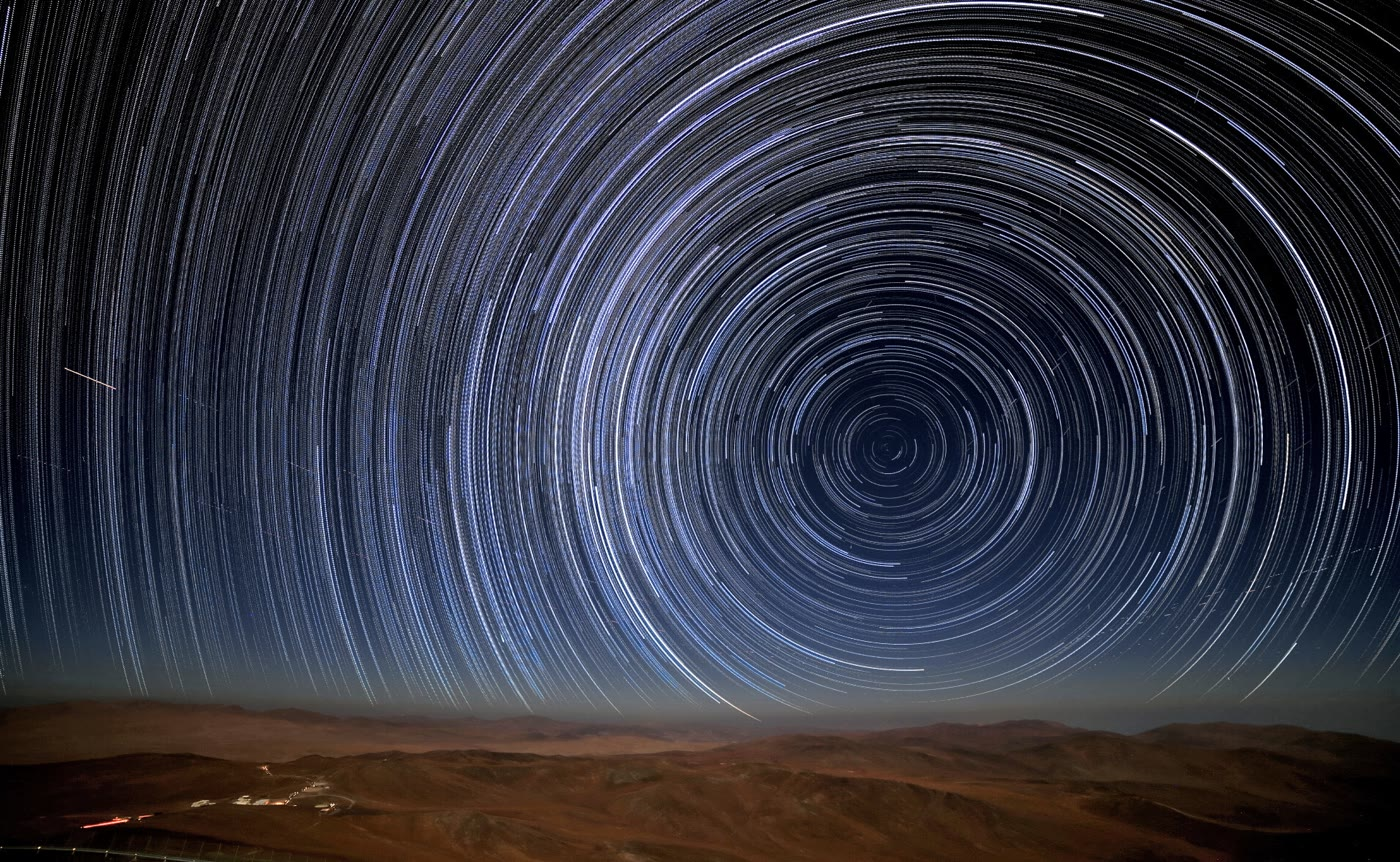
\includegraphics[width=0.8\linewidth]{images/book3/b1-star-trails-paranal.jpg}
% ledger: commons:eso-paranal-star-trails, mpc:paranal

{\small Traces d'étoiles au-dessus de l'observatoire du Paranal, dans le
désert d'Atacama, à la \omterm{def:b1:spherical-astronomy:geographic}{latitude} \ang{24.6}~S~: une longue pose enregistre
l'arc que décrit chaque étoile autour du \omterm{def:b1:spherical-astronomy:celestial-sphere}{pôle céleste} sud, qui se tient à
\ang{24.6} au-dessus de l'horizon sud. Photographie R.~Wesson/ESO, CC BY 4.0.}
\end{omfigure}

\section{Temps sidéral et temps solaire}

\begin{definition}[L'écliptique]\label{def:b1:spherical-astronomy:ecliptic}
L'\emph{écliptique}\index{ecliptique@écliptique} est le \omterm{def:b1:spherical-astronomy:spherical-triangle}{grand cercle} de la
\omterm{def:b1:spherical-astronomy:celestial-sphere}{sphère céleste} le long duquel le Soleil semble se déplacer en un an, trace du
plan de l'orbite de la Terre. Il est incliné sur l'\omterm{def:b1:spherical-astronomy:celestial-sphere}{équateur céleste} de
l'\emph{obliquité de l'écliptique}\index{obliquite de l'ecliptique@obliquité de l'écliptique}
$\varepsilon$, inclinaison de l'axe de la Terre sur son orbite. L'écliptique
coupe l'équateur en deux points~; le \emph{point vernal}\index{point vernal} $\gamma$ est
celui où le Soleil traverse l'équateur vers le nord, en mars. La \omterm{def:b1:spherical-astronomy:geographic}{longitude}
écliptique du Soleil $\lambda_\odot$ est son angle le long de l'écliptique
depuis $\gamma$, compté vers l'est.
\end{definition}

% ledger: earth:obliquity (23.44)
L'obliquité vaut aujourd'hui $\varepsilon = \ang{23.44}$.

\begin{definition}[Le temps sidéral]\label{def:b1:spherical-astronomy:sidereal-time}
Le \emph{temps sidéral}\index{temps sideral@temps sidéral} local est l'\omterm{def:b1:spherical-astronomy:equatorial}{angle horaire} du \omterm{def:b1:spherical-astronomy:ecliptic}{point vernal} $\gamma$. Un
jour sidéral est l'intervalle entre deux passages de $\gamma$ au méridien.
\end{definition}

Comme l'\omterm{def:b1:spherical-astronomy:equatorial}{ascension droite} est comptée vers l'est depuis $\gamma$ et l'\omterm{def:b1:spherical-astronomy:equatorial}{angle
horaire} vers l'ouest depuis le méridien, pour toute étoile
\[
  H = \mathrm{LST} - \alpha ,
\]
où LST est le \omterm{def:b1:spherical-astronomy:sidereal-time}{temps sidéral} local (sigle de l'anglais «~local sidereal
time~»)~: une étoile traverse le méridien quand le \omterm{def:b1:spherical-astronomy:sidereal-time}{temps sidéral} égale son
\omterm{def:b1:spherical-astronomy:equatorial}{ascension droite}. Une horloge d'observatoire indiquant le \omterm{def:b1:spherical-astronomy:sidereal-time}{temps sidéral} dit
d'un coup d'œil quelle région du ciel se trouve à la verticale.

\begin{proposition}[Jour sidéral et jour solaire]\label{prop:b1:spherical-astronomy:sidereal-day}
En une \omterm{def:b1:spherical-astronomy:tropical-year}{année tropique} de $N$ jours solaires moyens, la Terre fait $N + 1$ tours
par rapport aux étoiles. Le jour sidéral dure donc
\[
  \frac{N}{N + 1}\times\qty{24}{h},
\]
et avec $N = 365.2422$ cela fait \qty{23}{h}~\qty{56}{min}~\qty{4.09}{s}~: une
étoile traverse le méridien chaque jour \qty{3}{min}~\qty{56}{s} de \omterm{def:b1:spherical-astronomy:solar-time}{temps
solaire moyen} plus tôt.
\end{proposition}

\begin{proof}
% ledger: usno:tropical-year, earth:Trot (23.9345 h)
On compte les tours par rapport au Soleil et par rapport aux étoiles sur une
année. Le Soleil fait un tour de l'\omterm{def:b1:spherical-astronomy:ecliptic}{écliptique} vers l'est en un an, dans le
sens de la rotation de la Terre. Par rapport au Soleil, la Terre fait donc un
tour de moins que par rapport aux étoiles~: $N$ jours solaires et $N + 1$ jours
sidéraux remplissent la même année. Le jour sidéral est les $N/(N+1)$ d'un
jour solaire, soit
$\qty{86400}{s}\times 365.2422/366.2422 = \qty{86164.09}{s}$~; la différence
est de $\qty{235.9}{s}$. Cela s'accorde avec la période de rotation de la
Terre mesurée par rapport aux étoiles, \qty{23.9345}{h}.
\end{proof}

\begin{definition}[Le temps solaire]\label{def:b1:spherical-astronomy:solar-time}
Le \emph{temps solaire vrai}\index{temps solaire vrai} est l'\omterm{def:b1:spherical-astronomy:equatorial}{angle horaire} du
Soleil augmenté de 12 heures~: un cadran solaire l'indique, et il est midi
lorsque le Soleil traverse le méridien. Le \emph{temps solaire
moyen}\index{temps solaire moyen} est l'\omterm{def:b1:spherical-astronomy:equatorial}{angle horaire}, augmenté de 12 heures,
d'un Soleil moyen fictif qui se déplace sur l'\omterm{def:b1:spherical-astronomy:celestial-sphere}{équateur céleste} à vitesse
uniforme et fait un tour en une \omterm{def:b1:spherical-astronomy:tropical-year}{année tropique}. Leur différence, temps vrai
moins temps moyen, est l'\emph{équation du temps}\index{equation du temps@équation du temps}.
\end{definition}

Le Soleil vrai avance puis retarde sur le Soleil moyen, pour deux raisons. La
Terre va plus vite près du périhélie, début janvier, que près de l'aphélie, de
sorte que la progression du Soleil le long de l'\omterm{def:b1:spherical-astronomy:ecliptic}{écliptique} est inégale (deuxième
loi de Kepler)~; et le Soleil se déplace le long de l'\omterm{def:b1:spherical-astronomy:ecliptic}{écliptique}, qui est
inclinée sur l'équateur, de sorte que même un mouvement uniforme le long de
l'\omterm{def:b1:spherical-astronomy:ecliptic}{écliptique} se projette de façon inégale sur l'équateur --- ce que mesure
l'\omterm{def:b1:spherical-astronomy:equatorial}{angle horaire} --- plus vite près des solstices que près des équinoxes. Les
horloges civiles suivent le \omterm{def:b1:spherical-astronomy:solar-time}{temps solaire moyen} d'un méridien de référence de
leur fuseau horaire~; le temps moyen local à la \omterm{def:b1:spherical-astronomy:geographic}{longitude} $\lambda$ est en
avance sur celui de Greenwich de $\lambda/\ang{15}$ heures.

\begin{omfigure}
\begin{tikzpicture}
\begin{axis}[omrecord, width=0.9\linewidth, height=5.2cm, xmin=0, xmax=365,
  xtick={0,31,59,90,120,151,181,212,243,273,304,334,365},
  xticklabels={J,F,M,A,M,J,J,A,S,O,N,D,},
  ylabel={équation du temps (min)}, ymin=-20, ymax=21,
  tick label style={font=\scriptsize}, label style={font=\small}]
\addplot[black!50, line width=0.4pt] coordinates {(0,0) (365,0)};
\addplot[omDef, line width=1.1pt] table[x=day, y=eot_min] {figdata/out/bachelor-1-day_length-eot.dat};
\node[font=\scriptsize, above, fill=white, inner sep=1pt] at (axis cs:306,16.6) {$+16.4$};
\node[font=\scriptsize, below, fill=white, inner sep=1pt] at (axis cs:41,-14.4) {$-14.2$};
\end{axis}
\end{tikzpicture}

{\small L'\omterm{def:b1:spherical-astronomy:solar-time}{équation du temps} au cours de l'année (\omterm{def:b1:spherical-astronomy:solar-time}{temps solaire vrai} moins \omterm{def:b1:spherical-astronomy:solar-time}{temps
solaire moyen})~: un cadran solaire avance de \qty{16.4}{min} au plus début
novembre et retarde de \qty{14.2}{min} à la mi-février. Calculée à partir d'une
orbite képlérienne d'excentricité 0.0167, d'obliquité \ang{23.44}, avec la
\omterm{def:b1:spherical-astronomy:geographic}{longitude} du périhélie et la date de l'équinoxe de mars 2026.}
% ledger: earth:ecc, earth:obliquity, nasa:earth-perihelion-longitude, usno:seasons-2026
\end{omfigure}

\section{Lever, coucher et Soleil}

\begin{proposition}[Lever et coucher]\label{prop:b1:spherical-astronomy:rising}
À la \omterm{def:b1:spherical-astronomy:geographic}{latitude} $\varphi$, une étoile de \omterm{def:b1:spherical-astronomy:equatorial}{déclinaison} $\delta$ qui se lève et se
couche traverse l'horizon aux \omterm{def:b1:spherical-astronomy:equatorial}{angles horaires} $\pm H_0$ avec
\[
  \cos H_0 = -\tan\varphi\tan\delta ,
\]
à l'\omterm{def:b1:spherical-astronomy:horizontal}{azimut} $\mathrm{A}_0$ tel que $\cos\mathrm{A}_0 = \sin\delta/\cos\varphi$
(au lever~; elle se couche à $\ang{360} - \mathrm{A}_0$). Elle reste au-dessus
de l'horizon pendant $2H_0$, converti en heures à raison de \ang{15} par heure.
\end{proposition}

\begin{proof}
À l'horizon, $h = 0$, et la \cref{prop:b1:spherical-astronomy:transform}
donne $0 = \sin\varphi\sin\delta + \cos\varphi\cos\delta\cos H_0$, et
$\cos\mathrm{A}_0 = \sin\delta/\cos\varphi$. L'\omterm{def:b1:spherical-astronomy:equatorial}{angle horaire} croît
uniformément, de \ang{15} par heure, de $-H_0$ au lever à $+H_0$ au coucher.
\end{proof}

Pour le Soleil, cela donne la durée du jour, si l'on traite le Soleil comme un
point et que l'on néglige la réfraction de la lumière par l'air (l'un et
l'autre ajoutent quelques minutes de jour). Aux équinoxes, $\delta = 0$,
$H_0 = \ang{90}$~: le jour et la nuit durent douze heures partout, et le Soleil
se lève plein est.

\begin{omfigure}
\begin{tikzpicture}
\begin{axis}[omrecord, width=0.85\linewidth, height=5.6cm, xmin=40, xmax=320, ymin=0, ymax=75,
  xtick={45,90,135,180,225,270,315}, xticklabels={NE,E,SE,S,SO,O,NO}, ytick={0,15,30,45,60,75},
  xlabel={azimut}, ylabel={hauteur du Soleil ($^\circ$)},
  tick label style={font=\scriptsize}, label style={font=\small}]
\addplot[omThm, line width=1pt] table[x=az_deg, y=alt_deg] {figdata/out/bachelor-1-sun_paths-june.dat};
\addplot[black, line width=1pt] table[x=az_deg, y=alt_deg] {figdata/out/bachelor-1-sun_paths-equinox.dat};
\addplot[omDef, line width=1pt] table[x=az_deg, y=alt_deg] {figdata/out/bachelor-1-sun_paths-december.dat};
\begin{scope}[font=\scriptsize, fill=white, fill opacity=0.8, text opacity=1, inner sep=1pt]
  \node[omThm, above, fill=white] at (axis cs:180,68.4) {solstice de juin, $\ang{68.4}$};
  \node[above, fill=white] at (axis cs:180,45) {équinoxes, $\ang{45}$};
  \node[omDef, above, fill=white] at (axis cs:180,21.6) {solstice de décembre, $\ang{21.6}$};
\end{scope}
\end{axis}
\end{tikzpicture}

{\small La trajectoire du Soleil dans le ciel à la \omterm{def:b1:spherical-astronomy:geographic}{latitude} \ang{45}~N au
solstice de juin (en rouge), aux équinoxes (en noir) et au solstice de
décembre (en bleu), avec les \omterm{def:b1:spherical-astronomy:horizontal}{hauteurs} méridiennes
$\ang{90} - \varphi + \delta_\odot$. Aux équinoxes, le Soleil se lève plein est
et se couche plein ouest~; en juin, il se lève au nord-est.}
\end{omfigure}

\begin{proposition}[Déclinaison du Soleil]\label{prop:b1:spherical-astronomy:sun-declination}
Lorsque le Soleil est à la \omterm{def:b1:spherical-astronomy:geographic}{longitude} \omterm{def:b1:spherical-astronomy:ecliptic}{écliptique} $\lambda_\odot$, sa \omterm{def:b1:spherical-astronomy:equatorial}{déclinaison}
et son \omterm{def:b1:spherical-astronomy:equatorial}{ascension droite} vérifient
\[
  \sin\delta_\odot = \sin\varepsilon\sin\lambda_\odot, \qquad
  \tan\alpha_\odot = \cos\varepsilon\tan\lambda_\odot .
\]
\end{proposition}

\begin{proof}
Prenons des axes avec $x$ vers $\gamma$ et $z$ vers le \omterm{def:b1:spherical-astronomy:celestial-sphere}{pôle céleste} nord.
Dans des axes $x$, $y'$, $z'$ liés à l'\omterm{def:b1:spherical-astronomy:ecliptic}{écliptique}, avec $z'$ vers son pôle,
la direction du Soleil est $(\cos\lambda_\odot, \sin\lambda_\odot, 0)$. Les
axes de l'\omterm{def:b1:spherical-astronomy:ecliptic}{écliptique} sont ceux de l'équateur tournés de l'angle $\varepsilon$
autour de $x$, donc dans les axes équatoriaux la direction du Soleil est
$(\cos\lambda_\odot,\ \sin\lambda_\odot\cos\varepsilon,\
\sin\lambda_\odot\sin\varepsilon)$. Sa composante en $z$ est
$\sin\delta_\odot$~; le rapport de ses composantes en $y$ et en $x$ est
$\tan\alpha_\odot$.
\end{proof}

\begin{omfigure}
\begin{tikzpicture}
\begin{axis}[omrecord, width=0.9\linewidth, height=6cm, xmin=0, xmax=365, ymin=0, ymax=24,
  xtick={0,31,59,90,120,151,181,212,243,273,304,334,365},
  xticklabels={J,F,M,A,M,J,J,A,S,O,N,D,}, ytick={0,6,12,18,24},
  ylabel={durée du jour (h)}, tick label style={font=\scriptsize}, label style={font=\small},
  legend style={font=\scriptsize, at={(0.5,1.02)}, anchor=south, draw=none}, legend columns=5,
  legend cell align=left]
\addplot[black, line width=0.9pt] table[x=day, y=lat0] {figdata/out/bachelor-1-day_length-lengths.dat};
\addplot[omDef, line width=0.9pt] table[x=day, y=lat30] {figdata/out/bachelor-1-day_length-lengths.dat};
\addplot[omThm, line width=0.9pt] table[x=day, y=lat45] {figdata/out/bachelor-1-day_length-lengths.dat};
\addplot[omField, line width=0.9pt] table[x=day, y=lat60] {figdata/out/bachelor-1-day_length-lengths.dat};
\addplot[black, line width=0.9pt, densely dashed] table[x=day, y=lat70] {figdata/out/bachelor-1-day_length-lengths.dat};
\legend{\ang{0}, \ang{30}~N, \ang{45}~N, \ang{60}~N, \ang{70}~N}
\end{axis}
\end{tikzpicture}

{\small Durée du jour (centre du Soleil au-dessus de l'horizon géométrique) au
cours de l'année à cinq \omterm{def:b1:spherical-astronomy:geographic}{latitudes} nord, d'après les
\cref{prop:b1:spherical-astronomy:rising,prop:b1:spherical-astronomy:sun-declination}.
À \ang{70}~N, le Soleil reste levé pendant des semaines autour du solstice de
juin et reste couché autour du solstice de décembre. Dans l'hémisphère sud, les
courbes sont décalées d'une demi-année.}
\end{omfigure}

\begin{definition}[Insolation]\label{def:b1:spherical-astronomy:insolation}
L'\emph{insolation}\index{insolation} en un lieu et à un instant est la
puissance de la lumière solaire reçue par unité de surface d'une surface
horizontale au sommet de l'atmosphère. Avec $S_0$ l'irradiance solaire à la
distance moyenne $a$ du Soleil, $r$ la distance réelle et $\theta_z$ la
distance zénithale du Soleil,
\[
  I = S_0\left(\frac{a}{r}\right)^{2}\cos\theta_z = S_0\left(\frac{a}{r}\right)^{2}\sin h_\odot
  \quad (h_\odot > 0), \qquad I = 0 \text{ la nuit}.
\]
\end{definition}

% ledger: earth:TSI (1361 W/m2), earth:peri, earth:aph, earth:a
Le facteur $(a/r)^2$ est la loi en inverse du carré de la distance pour la
lumière (les livres de physique)~; le facteur $\cos\theta_z$ apparaît parce
qu'un faisceau de section un mètre carré s'étale sur $1/\cos\theta_z$ mètres
carrés de sol horizontal. Avec
$S_0 = \qty{1361}{W.m^{-2}}$ et une distance Soleil--Terre comprise entre
\qty{147.1e6}{km} au périhélie et \qty{152.1e6}{km} à l'aphélie, le facteur
$(a/r)^2$ varie de $\pm\qty{3.4}{\percent}$ au cours de l'année. L'inclinaison
de l'axe fait beaucoup plus~: elle modifie à la fois la \omterm{def:b1:spherical-astronomy:horizontal}{hauteur} du Soleil à
midi et la durée du jour, et ces deux effets réunis font les saisons. Les
sommes journalière et annuelle de l'\omterm{def:b1:spherical-astronomy:insolation}{insolation}, qui pilotent le climat, sont
calculées au \cref{ch:b1:radiation-heat-transport}.


\section{Calendriers}

\begin{definition}[L'année tropique]\label{def:b1:spherical-astronomy:tropical-year}
L'\emph{année tropique}\index{annee tropique@année tropique} est l'intervalle moyen entre deux passages du Soleil
au \omterm{def:b1:spherical-astronomy:ecliptic}{point vernal}. Elle gouverne les saisons~; elle dure 365.2422 jours solaires
moyens.
\end{definition}

% ledger: usno:tropical-year, earth:Psid (365.256 d)
L'\omterm{def:b1:spherical-astronomy:tropical-year}{année tropique} est plus courte d'environ vingt minutes que l'année sidérale,
temps que met la Terre à revenir au même endroit parmi les étoiles
(365.256 jours), parce que l'axe de la Terre tourne lentement --- il
précesse --- et entraîne le \omterm{def:b1:spherical-astronomy:ecliptic}{point vernal} à rebours le long de l'\omterm{def:b1:spherical-astronomy:ecliptic}{écliptique} (le
volume de deuxième année). Un calendrier doit faire tenir un nombre entier de
jours dans l'\omterm{def:b1:spherical-astronomy:tropical-year}{année tropique}, afin que les saisons reviennent aux mêmes dates.

\begin{proposition}[L'année grégorienne]\label{prop:b1:spherical-astronomy:gregorian}
Dans le calendrier grégorien, une année est bissextile (366 jours) si son
millésime est divisible par 4, sauf les années séculaires, qui ne sont
bissextiles que si leur millésime est divisible par 400. L'année moyenne vaut
\[
  365 + \frac14 - \frac1{100} + \frac1{400} = \num{365.2425}\text{ jours},
\]
et elle dérive par rapport aux saisons d'un jour en 3300 ans environ.
\end{proposition}

\begin{proof}
% ledger: usno:leap-rule, usno:tropical-year
En 400 ans, il y a 100 années divisibles par 4~; parmi elles figurent quatre
années séculaires, dont trois ne sont pas divisibles par 400. Il y a donc 97
années bissextiles et $400\times 365 + 97 = 146\,097$ jours,
soit 365.2425 jours par an. Par rapport à une \omterm{def:b1:spherical-astronomy:tropical-year}{année tropique} de 365.2422 jours,
l'excès est de 0.0003 jour par an~: un jour en $1/0.0003 \approx 3300$ ans.
\end{proof}

\begin{history}[La réforme de 1582]
% ledger: usno:gregorian-1582
Le calendrier julien, hérité de Rome, ajoutait un jour bissextile tous les
quatre ans~: son année de 365.25 jours dépasse l'\omterm{def:b1:spherical-astronomy:tropical-year}{année tropique} de 0.0078 jour,
soit un jour en 128 ans. Au fil des siècles, la date de l'équinoxe de printemps
s'éloigna du 21 mars, date sur laquelle reposait le calcul de Pâques. En 1582,
le pape Grégoire~XIII introduisit le calendrier qui porte son nom~: il supprima
d'un coup les jours accumulés et remplaça la règle julienne par celle de la
\cref{prop:b1:spherical-astronomy:gregorian}. C'est devenu le calendrier civil
admis dans le monde entier.
\end{history}

\begin{inthefield}[Se repérer grâce aux étoiles]
Avant le positionnement par satellite, les navigateurs en mer déterminaient
leur \omterm{def:b1:spherical-astronomy:geographic}{latitude} et leur \omterm{def:b1:spherical-astronomy:geographic}{longitude} d'après le ciel. Au sextant, ils mesuraient la
\omterm{def:b1:spherical-astronomy:horizontal}{hauteur} du Soleil à midi, ou celle de deux ou trois étoiles au crépuscule, et
lisaient l'heure sur un chronomètre réglé sur le temps du méridien de
Greenwich. Chaque \omterm{def:b1:spherical-astronomy:horizontal}{hauteur}, avec la \omterm{def:b1:spherical-astronomy:equatorial}{déclinaison} de l'astre et son \omterm{def:b1:spherical-astronomy:equatorial}{angle horaire}
à Greenwich tirés d'un almanach, donne un \omterm{def:b1:spherical-astronomy:spherical-triangle}{petit cercle} sur la Terre où se
trouve le navire~: le cercle des points d'où l'astre est vu à cette \omterm{def:b1:spherical-astronomy:horizontal}{hauteur}.
Deux ou trois de ces cercles se coupent à la position du navire --- de la
trigonométrie sphérique résolue en mer chaque jour. La seule \omterm{def:b1:spherical-astronomy:horizontal}{hauteur} du Soleil
à midi donne la \omterm{def:b1:spherical-astronomy:geographic}{latitude} (\cref{prop:b1:spherical-astronomy:culmination})~;
l'heure de l'horloge au midi local donne la \omterm{def:b1:spherical-astronomy:geographic}{longitude}, à raison de quatre
minutes de temps par degré.
\begin{center}
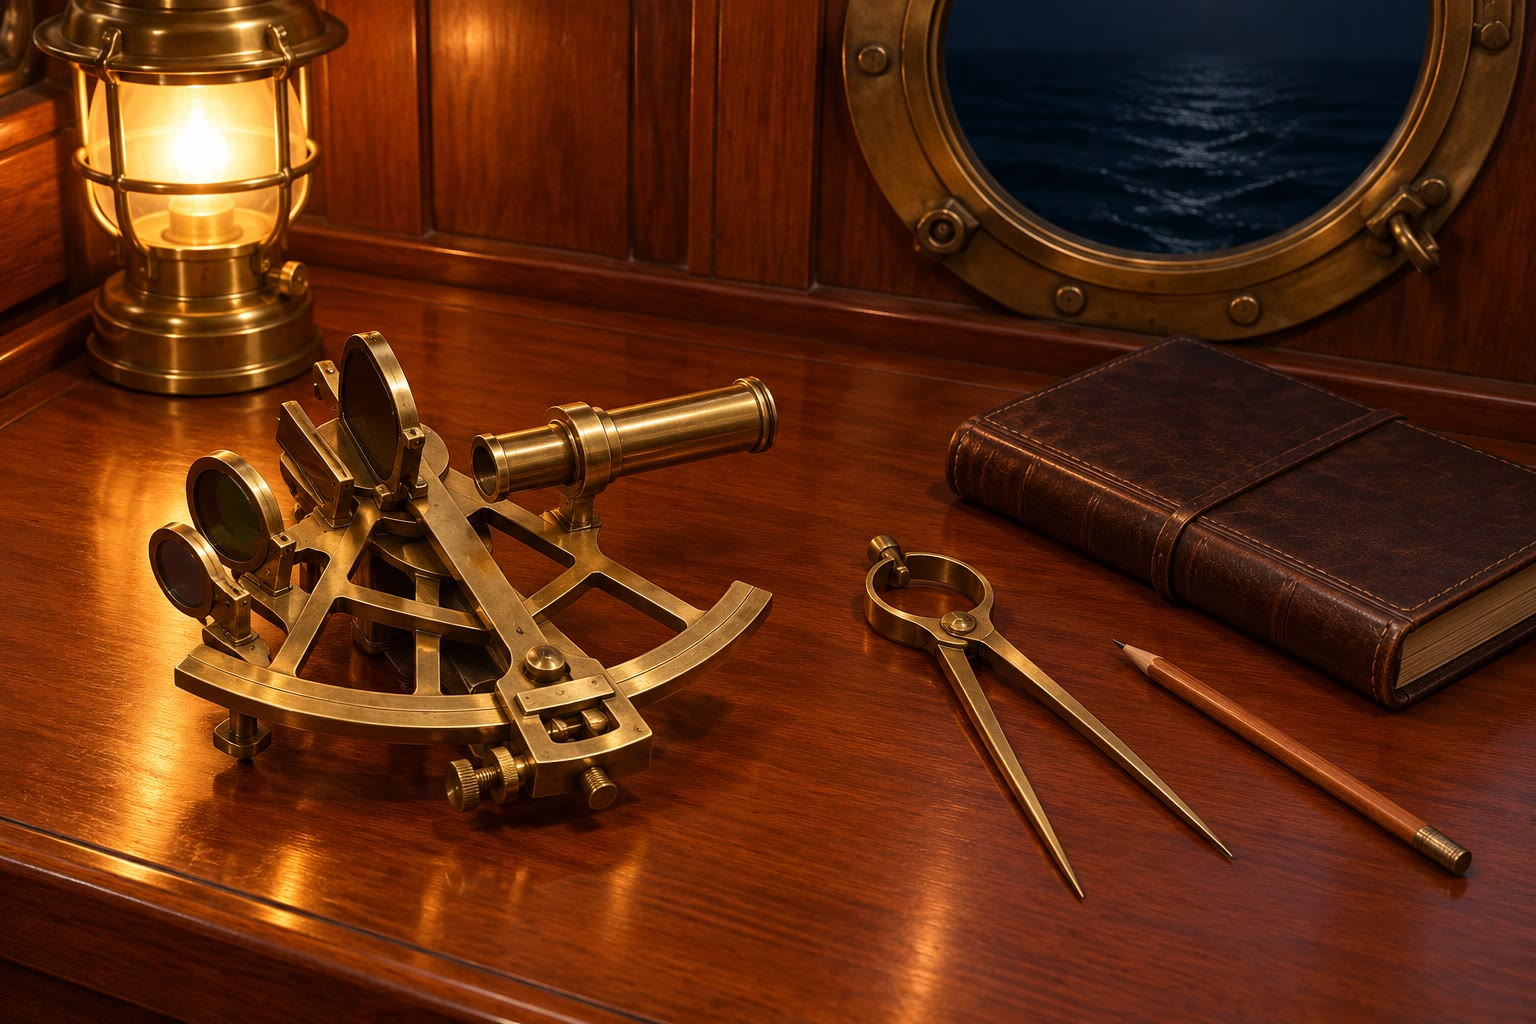
\includegraphics[width=0.55\linewidth]{images/book3/ai/b1-sextant.jpg}
\end{center}
\end{inthefield}

\section{Exercices}

\begin{exercise}[$\star$]\label{exo:b1:spherical-astronomy:1}
Un observateur se trouve à la \omterm{def:b1:spherical-astronomy:geographic}{latitude} \ang{52}~N. À quelle \omterm{def:b1:spherical-astronomy:horizontal}{hauteur} se tient le
\omterm{def:b1:spherical-astronomy:celestial-sphere}{pôle céleste} nord~? Quelles étoiles, d'après leur \omterm{def:b1:spherical-astronomy:equatorial}{déclinaison}, ne se couchent
jamais en ce lieu, et lesquelles ne s'y lèvent jamais~?
\end{exercise}

\begin{exercise}[$\star$]\label{exo:b1:spherical-astronomy:2}
Convertir en degrés une \omterm{def:b1:spherical-astronomy:equatorial}{ascension droite} de \qty{6}{h}~\qty{45}{min}. Pour un
\omterm{def:b1:spherical-astronomy:sidereal-time}{temps sidéral} local de \qty{10}{h}~\qty{0}{min}, quel est l'\omterm{def:b1:spherical-astronomy:equatorial}{angle horaire} d'une
étoile de cette \omterm{def:b1:spherical-astronomy:equatorial}{ascension droite}~? L'étoile est-elle à l'est ou à l'ouest du
méridien~?
\end{exercise}

\begin{exercise}[$\star$]\label{exo:b1:spherical-astronomy:3}
À la \omterm{def:b1:spherical-astronomy:geographic}{latitude} \ang{40}~N, calculer la \omterm{def:b1:spherical-astronomy:horizontal}{hauteur} du Soleil à midi aux deux
solstices et aux équinoxes ($\varepsilon = \ang{23.44}$).
\end{exercise}

\begin{exercise}[$\star$]\label{exo:b1:spherical-astronomy:4}
L'année 1900 était-elle bissextile~? Et 2000~? Et 2100, le sera-t-elle~? De
combien de jours par siècle le calendrier julien dérive-t-il par rapport à une
\omterm{def:b1:spherical-astronomy:tropical-year}{année tropique} de 365.2422 jours, et de combien le calendrier grégorien~?
\end{exercise}

\begin{exercise}[$\star\star$]\label{exo:b1:spherical-astronomy:5}
Deux points sont situés à la \omterm{def:b1:spherical-astronomy:geographic}{latitude} \ang{45}~N, aux \omterm{def:b1:spherical-astronomy:geographic}{longitudes} \ang{0} et
\ang{90}~E. Calculer la distance orthodromique qui les sépare
($R = \qty{6371}{km}$) et la distance le long de leur parallèle. Laquelle est
la plus courte, et de combien~?
\end{exercise}

\begin{exercise}[$\star\star$]\label{exo:b1:spherical-astronomy:6}
À la \omterm{def:b1:spherical-astronomy:geographic}{latitude} \ang{48}~N, une étoile de \omterm{def:b1:spherical-astronomy:equatorial}{déclinaison} \ang{20} a pour \omterm{def:b1:spherical-astronomy:equatorial}{angle
horaire} \ang{30}. Calculer sa \omterm{def:b1:spherical-astronomy:horizontal}{hauteur} et son \omterm{def:b1:spherical-astronomy:horizontal}{azimut}. Dans quelle direction
l'observateur doit-il regarder~?
\end{exercise}

\begin{exercise}[$\star\star$]\label{exo:b1:spherical-astronomy:7}
Calculer la durée du jour à la \omterm{def:b1:spherical-astronomy:geographic}{latitude} \ang{60}~N au solstice de juin, le
Soleil étant traité comme un point sur un horizon géométrique. Vérifier le
résultat sur la figure des durées du jour.
\end{exercise}

\begin{exercise}[$\star\star$]\label{exo:b1:spherical-astronomy:8}
Une étoile traverse le méridien ce soir à 22~h, temps moyen local. À quelle
heure le traversera-t-elle dans 30 jours~? Dans combien de jours le
traversera-t-elle à midi, invisible en plein jour~?
\end{exercise}

\begin{exercise}[$\star\star$]\label{exo:b1:spherical-astronomy:9}
Calculer l'\omterm{def:b1:spherical-astronomy:insolation}{insolation} au sommet de l'atmosphère à midi à la \omterm{def:b1:spherical-astronomy:geographic}{latitude}
\ang{45}~N (a) à un équinoxe, en prenant $r = a$~; (b) au solstice de juin, en
prenant pour $r$ la distance à l'aphélie. Données~: $S_0 = \qty{1361}{W.m^{-2}}$,
$a = \qty{149.598e6}{km}$, aphélie \qty{152.100e6}{km}.
\end{exercise}

\begin{exercise}[$\star\star\star$]\label{exo:b1:spherical-astronomy:10}
À l'aide de la \cref{prop:b1:spherical-astronomy:sun-declination}, calculer la
\omterm{def:b1:spherical-astronomy:equatorial}{déclinaison} et l'\omterm{def:b1:spherical-astronomy:equatorial}{ascension droite} du Soleil lorsque sa \omterm{def:b1:spherical-astronomy:geographic}{longitude} \omterm{def:b1:spherical-astronomy:ecliptic}{écliptique}
vaut \ang{60}. De combien de degrés l'\omterm{def:b1:spherical-astronomy:equatorial}{ascension droite} est-elle en retard sur
la \omterm{def:b1:spherical-astronomy:geographic}{longitude}~? Expliquer, à l'aide de ce résultat, pourquoi l'inclinaison de
l'\omterm{def:b1:spherical-astronomy:ecliptic}{écliptique} contribue à l'\omterm{def:b1:spherical-astronomy:solar-time}{équation du temps}.
\end{exercise}

\begin{exercise}[$\star\star\star$]\label{exo:b1:spherical-astronomy:11}
Montrer qu'au solstice de juin le Soleil se lève à l'\omterm{def:b1:spherical-astronomy:horizontal}{azimut} $\mathrm{A}_0$
tel que $\cos\mathrm{A}_0 = \sin\varepsilon/\cos\varphi$. À quelle \omterm{def:b1:spherical-astronomy:geographic}{latitude} se
lève-t-il exactement au nord-est~? Que devient la formule aux \omterm{def:b1:spherical-astronomy:geographic}{latitudes}
supérieures à $\ang{90} - \varepsilon$~?
\end{exercise}

\begin{exercise}[$\star\star\star$]\label{exo:b1:spherical-astronomy:12}
Un fuseau sphérique est la partie d'une sphère comprise entre deux demi-grands
cercles joignant deux points opposés et faisant entre eux l'angle $\theta$.
(a) Montrer que son aire est $2\theta R^2$. (b) Chaque côté d'un \omterm{def:b1:spherical-astronomy:spherical-triangle}{triangle
sphérique} $ABC$, prolongé en un \omterm{def:b1:spherical-astronomy:spherical-triangle}{grand cercle} entier, donne avec les autres trois
paires de fuseaux opposés d'angles $A$, $B$, $C$ qui recouvrent la sphère, le
triangle et son opposé étant recouverts trois fois. En déduire le théorème de
Girard~: l'aire du triangle est $R^2(A + B + C - \pi)$. (c) L'appliquer au
triangle à trois angles droits, et au triangle dessiné dans ce chapitre (angles
\ang{89.9}, \ang{64.9}, \ang{67.4}).
\end{exercise}

\section{Problème~: Une nuit dans un observatoire de montagne}

\begin{problem}[{Problème du week-end --- où se trouve l'observatoire du Paranal, ce que
montre son ciel et combien de temps dure sa plus longue nuit}]
\label{pb:b1:spherical-astronomy:1}
% ledger: mpc:paranal, mpc:greenwich, simbad:sirius, simbad:canopus, usno:seasons-2026, earth:obliquity, usno:tropical-year
% numbers computed in the scratch calculator calc/ch01.py from the rounded data
L'observatoire du Paranal se dresse dans le désert d'Atacama, à la \omterm{def:b1:spherical-astronomy:geographic}{latitude}
\ang{24.63}~S et à la \omterm{def:b1:spherical-astronomy:geographic}{longitude} \ang{70.40}~O. L'observatoire royal de
Greenwich, par lequel on compte les \omterm{def:b1:spherical-astronomy:geographic}{longitudes}, est à \ang{51.48}~N,
\ang{0.00}. Deux étoiles brillantes du ciel austral ont pour coordonnées
\begin{center}
\small
\begin{tabular}{lcc}
\hline
étoile & \omterm{def:b1:spherical-astronomy:equatorial}{ascension droite} & \omterm{def:b1:spherical-astronomy:equatorial}{déclinaison} \\
\hline
Sirius & \qty{6}{h}~\qty{45}{min}~\qty{9}{s} & \ang{-16.72} \\
Canopus & \qty{6}{h}~\qty{23}{min}~\qty{57}{s} & \ang{-52.70} \\
\hline
\end{tabular}
\end{center}
On prend $R = \qty{6371}{km}$, $\varepsilon = \ang{23.44}$, une \omterm{def:b1:spherical-astronomy:tropical-year}{année tropique}
de 365.2422 jours, et l'on traite le Soleil comme un point sur un horizon
géométrique.

\medskip
\noindent\textbf{Partie I --- Le Paranal sur le globe.}
\begin{enumerate}
  \item Donner les colatitudes du Paranal et de Greenwich, et leur différence
        de \omterm{def:b1:spherical-astronomy:geographic}{longitude}.
  \item Écrire la formule des cosinus pour le triangle pôle Nord--Paranal--Greenwich
        et calculer le cosinus de la distance angulaire $\Delta$ entre les
        deux observatoires.
  \item En déduire $\Delta$ en degrés et la distance orthodromique en
        kilomètres.
  \item Calculer le cap initial du Paranal vers Greenwich
        (\cref{met:b1:spherical-astronomy:great-circle}).
  \item Vérifier le cap avec la formule des sinus.
  \item Un avion qui garderait ce cap jusqu'au bout atteindrait-il Greenwich~?
        Expliquer.
\end{enumerate}

\medskip
\noindent\textbf{Partie II --- Le ciel du Paranal.}
\begin{enumerate}[resume]
  \item À quelle \omterm{def:b1:spherical-astronomy:horizontal}{hauteur} le \omterm{def:b1:spherical-astronomy:celestial-sphere}{pôle céleste} sud se tient-il au-dessus de
        l'horizon sud du Paranal~?
  \item À quelle \omterm{def:b1:spherical-astronomy:horizontal}{hauteur} Sirius traverse-t-il le méridien, et de quel côté du
        \omterm{def:b1:spherical-astronomy:celestial-sphere}{zénith}~?
  \item Au-dessous de quelle \omterm{def:b1:spherical-astronomy:equatorial}{déclinaison} une étoile est-elle circumpolaire au
        Paranal~? Canopus est-il circumpolaire~?
  \item Quelle est la plus grande \omterm{def:b1:spherical-astronomy:horizontal}{hauteur} que Canopus atteigne~?
  \item Calculer l'\omterm{def:b1:spherical-astronomy:equatorial}{angle horaire} auquel Sirius se lève, et combien de temps il
        reste au-dessus de l'horizon, en heures sidérales.
  \item À quel \omterm{def:b1:spherical-astronomy:horizontal}{azimut} Sirius se lève-t-il~?
\end{enumerate}

\medskip
\noindent\textbf{Partie III --- Horloges.}
\begin{enumerate}[resume]
  \item Quel est le \omterm{def:b1:spherical-astronomy:sidereal-time}{temps sidéral} local lorsque Sirius traverse le méridien~?
  \item Calculer la durée du jour sidéral, et de combien de minutes le passage
        d'une étoile au méridien avance chaque nuit.
  \item On prend le \omterm{def:b1:spherical-astronomy:sidereal-time}{temps sidéral} local à minuit moyen local égal à
        \qty{12}{h} à l'équinoxe de mars (20 mars 2026), lorsque le Soleil est
        près du \omterm{def:b1:spherical-astronomy:ecliptic}{point vernal}~; il gagne ensuite $24/365.2422$ heures par jour.
        Combien de jours après l'équinoxe Sirius traverse-t-il le méridien à
        minuit moyen local~? À quelle date~?
  \item Cette nuit-là, de combien le temps moyen local du Paranal diffère-t-il
        de l'heure de Greenwich~?
  \item L'\omterm{def:b1:spherical-astronomy:solar-time}{équation du temps} vaut alors environ \qty{-3}{min}. Quelle heure
        indique un cadran solaire de l'observatoire (\omterm{def:b1:spherical-astronomy:solar-time}{temps solaire vrai})
        lorsque Sirius traverse le méridien~?
  \item De combien plus tôt le traverse-t-il une semaine plus tard~?
\end{enumerate}

\medskip
\noindent\textbf{Partie IV --- La plus longue nuit.}
\begin{enumerate}[resume]
  \item Quelle est la \omterm{def:b1:spherical-astronomy:equatorial}{déclinaison} du Soleil à chaque solstice~?
  \item Calculer la \omterm{def:b1:spherical-astronomy:horizontal}{hauteur} du Soleil à midi au Paranal aux solstices de juin et
        de décembre. De quel côté du \omterm{def:b1:spherical-astronomy:celestial-sphere}{zénith} se trouve-t-il en décembre~?
  \item Au solstice de décembre, la distance Soleil--Terre vaut 0.9837 fois la
        distance moyenne. Calculer l'\omterm{def:b1:spherical-astronomy:insolation}{insolation} à midi au sommet de
        l'atmosphère au-dessus du Paranal ($S_0 = \qty{1361}{W.m^{-2}}$).
  \item À quel solstice la nuit est-elle la plus longue au Paranal~? Calculer
        l'\omterm{def:b1:spherical-astronomy:equatorial}{angle horaire} du coucher du Soleil à cette date.
  \item À quel \omterm{def:b1:spherical-astronomy:horizontal}{azimut} le Soleil se lève-t-il à cette date~?
  \item En déduire la durée de la plus longue nuit de l'année au Paranal, en
        heures et minutes.
\end{enumerate}
\end{problem}
